\documentclass{report}

\usepackage[utf8]{inputenc}
\usepackage[nottoc]{tocbibind}
\usepackage{vhistory}
\usepackage[ampersand]{easylist}
\usepackage{natbib}
\usepackage{url}
\usepackage{scrextend}
\usepackage{graphicx}
\usepackage{multicol}
\usepackage[titletoc]{appendix}
\usepackage{float}
\usepackage{blindtext}
\usepackage{listings}
\usepackage{xcolor}
\usepackage{tabto} \NumTabs{3}
\usepackage{enumitem}
\usepackage{booktabs}
\usepackage{xspace}
\usepackage{tabularx}
\usepackage{caption}
\usepackage{hhline}
\usepackage{chngpage}
\usepackage{mathtools}

\DeclareCaptionLabelFormat{blank}{}

\graphicspath{ {img/} }

\begin{document}

\begin{titlepage}
	\centering
	
\includegraphics[width=0.5\textwidth]{polimi-logo}\par\vspace{1cm}
	{\scshape\LARGE Politecnico di Milano\par}
	\vspace{1cm}
	{\scshape\Large Software Engineering 2 project\par}
	\vspace{1.5cm}
	{\Huge\bfseries PowerEnJoy\par}
	\vspace{0.5cm}
	{\Large\bfseries Project Plan Document\par}
	\vspace{2cm}
	\begin{multicols}{2}
		{\Large\itshape Matteo Penco\par}
		\vspace{0.25cm}
		mat. 875740
		\vfill\columnbreak
		{\Large\itshape Riccardo Pressiani\par}
		\vspace{0.25cm}
		mat. 874948
	\end{multicols}
	
	\vfill
	
	{\Large Version 1.1 approved\par}
	\vspace{1.25cm}
	{\large \today\par}
\end{titlepage}

\begin{versionhistory}
	\vhEntry{0.1}{18.01.17}{RP}{Document created}
	\vhEntry{1.0}{22.01.17}{RP and MP}{Document approved}
	\vhEntry{1.1}{07.02.17}{MP}{Fix Gantt diagrams}
\end{versionhistory}

\vspace{5cm}
{\noindent\Huge\bfseries Hours of work\par}
\vspace{0.5cm}
{\noindent Matteo Penco	\tab{15h}\par}
{\noindent Riccardo Pressiani \tab{15h}\par}

\tableofcontents

%Introduction
\chapter{Introduction}

\section{Purpose}
This document provides a high detailed description about the design and the architecture of the PowerEnJoy software.
It includes the design information about the components and how they intereact among them, the design of the most complex algorithm and the user interface design of the software to be developed.

This document is inteded for the key design stakeholders, which include managers and the development team.

\section{Scope}
PowerEnJoy is inteded to be a management system for a car-sharing system that exclusively employs electrical powered cars.
The system allows users to find all the available cars near a given location which can be their current position or a specific address typed in. The user can book one of the cars available for a limited amount of time.
Once the booked car is reached by the user, it can be unlocked from one of the smart devices of the user. After entering a PIN, decided by the user during the registration phase, on the onboard computer, the engine can be started and the rental begins.
The cost of the service is calculated on the total duration of the rental multiplied by a fixed rate per minute. The user is continuously informed about the cost of the ongoing rental by the onboard computer.
The user can end the rental by parking the car and stopping the engine.

The PowerEnJoy platform is intended to be available on the major mobile devices, such as smartphones and tablets running iOS \cite{ios} or Android \cite{android}.
\section{Definitions, acronyms and abbreviations}

% \subsection{Definitions}
% 	\begin{labeling}{defs}
% 		\item[\textbf{TEST}] \blindtext
% 	\end{labeling}

\subsection{Acronyms}
	\begin{labeling}{acro}
		\item[\textbf{PIN}] Personal Identification Number
		\item[\textbf{RASD}] Requirement Analysis and Specification Document
	\end{labeling}

% \subsection{Abbreviations}
% 	\begin{labeling}{abbrv}
% 		\item[\textbf{TEST}] \blindtext
% 	\end{labeling}
\section{References}

\begin{itemize}
	\item Assigments document for the first semester project of the Software Engineering 2 course held at Politecnico di Milano by Mottola Luca and Di Nitto Elisabetta \cite{assignments}.
	\item PowerEnjoy - Requirement Analysis and Specification Document \cite{rasd}.
	\item IEEE Standard for Information Technology—Systems Design— Software Design Descriptions \cite{ieee_sdd}.
	\item IEEE Systems and software engineering — Architecture description \cite{ieee_arch}.
	\item IEEE Recommended Practice for Architectural Description of Software-Intensive Systems \cite{ieee1471}.
\end{itemize}

% !TEX root = ../../../main.tex

\section{Overview}

A general introduction about the PowerEnJoy project has been given in this chapter. In the following chapters the reader will be provided with a more detailed description of the integration testing procedures.

In Chapter 2, the entry criteria to begin the integration testing phase will be provided. Moreover, the strategy and the integration test order will be described.

In Chapter 3, a detailed description of each integration test will be provided. These descriptions will include the expected input values and the corresponding state after each method invocation.

In Chapter 4, tools and equipment used to perform the tests will be listed along with a brief description.

In Chapter 5, the drivers needed and the set of data used to perform the tests correctly will be described.


%Project size, cost and effort estimation
% !TEX root = ../../main.tex
\chapter{Project size, cost and effort estimation}
This chapter provides an estimation of the expected size, cost and required effort of the PowerEnJoy project.

The size estimation will be based on the Function Points approach. This approach estimates the size of a software project starting from the functionalities that it has to offer. It is important to state that only the business logic has been taken into account, while the user applications have not been included in the estimation.

The cost and effort estimation will be based on the COCOMO II approach, starting from the SLOC value obtained from the size estimation.

% !TEX root = ../../../main.tex
\section{Size estimation: Function Points}
\blindtext

\begin{table}[h!tb]
	\centering
	\caption{UFP Complexity Weights}
	\label{tab:ufp}
	\begin{tabular}{|c|c|c|c|}
		\hline
		 & \multicolumn{3}{ c |}{Complexity Weight}	\\	\hline
		\textit{Function type} & \textit{Low} & \textit{Average} & \textit{High}\\ \hline
		Internal Logic Files	& 7 & 10 & 15\\
		External Logic Files	& 5 & 7 & 10 \\
		External Inputs			& 3 & 4 & 6 \\
		External Outputs		& 4 & 5 & 7 \\
		External Inquiries		& 3 & 4 & 6 \\
		\hline
	\end{tabular}
\end{table}


\subsection{Internal Logic Files}
\blindtext

\begin{table}[h!tb]
	\centering
	\caption{ILFs Function Points}
	\label{tab:ilfs}
	\begin{tabular}{|l|l|l|}
		\hline
		ILF					&	Complexity	&	FPs	\\ \hline
		User data				&	Low		&	7	\\
		Car status				&	Low	    &	7	\\
		Safe areas	  			&   Low     &   7   \\ 
		Booking					&	Average &   10  \\
		Rental					&   Average &   10  \\ \hline
		\multicolumn{2}{| l |}{Total}		&	41\\
		\hline
	\end{tabular}
\end{table}

\subsection{External Logic Files}
\blindtext

\begin{table}[h!tb]
	\centering
	\caption{ELFs Function Points}
	\label{tab:elfs}
	\begin{tabular}{|l|l|l|}
		\hline
		ELF					&	Complexity	&	FPs	\\ \hline
		Recovery request	 &	 Low		&	5	\\
		Notification message &	 Low		&	5	\\
		Payment request		 &	 Low		&   5  \\ \hline
		\multicolumn{2}{| l |}{Total}		&	15\\
		\hline
	\end{tabular}
\end{table}

\subsection{External Inputs}
\blindtext

\begin{table}[h!tb]
	\centering
	\caption{EIs Function Points}
	\label{tab:eis}
	\begin{tabular}{|l|l|l|}
		\hline
		EI					&	Complexity	&	FPs	\\ \hline
		User registration	&	Average		&	4	\\
		Login/Logout		&	Low			&	2*3	\\ 
		Book a car			&	Average		&	4	\\
		Delete booking		&	Low			&	3	\\
		Unlock car doors	&	Average		&	4	\\
		Begin rental		&	High		&	6	\\
		End rental			&	High		&	6	\\ \hline
		\multicolumn{2}{| l |}{Total}		&	33\\
		\hline
	\end{tabular}
\end{table}

\subsection{External Inquiries}
\blindtext

\begin{table}[h!tb]
	\centering
	\caption{EQs Function Points}
	\label{tab:eqs}
	\begin{tabular}{|l|l|l|}
		\hline
		EQ					&	Complexity	&	FPs	\\ \hline
		Find cars						&	Low			&	3	\\
		Get details about car			&	Low			&	3	\\ 
		Get info about ongoing rental	&	High		&	6	\\ \hline
		\multicolumn{2}{| l |}{Total}					&	12\\
		\hline
	\end{tabular}
\end{table}

\subsection{External Outputs}
\blindtext

\begin{table}[h!tb]
	\centering
	\caption{EOs Function Points}
	\label{tab:eos}
	\begin{tabular}{|l|l|l|}
		\hline
		EO					&	Complexity	&	FPs	\\ \hline
		Elapsed booking notification		&	Low		&	4	\\
		Unlock car doors notification		&	Low		&	4	\\
		Ended rental notification			&	Low		&	4	\\ \hline
		\multicolumn{2}{| l |}{Total}					&	12\\
		\hline
	\end{tabular}
\end{table}

\subsection{Overall Estimation}
\blindtext

\begin{table}[h!tb]
	\centering
	\caption{Function Points overall estimation}
	\label{tab:overall_fps}
	\begin{tabular}{|l|l|}
		\hline
		Function Type		&	Value	\\ \hline
		Internal Logic Files	&	41	\\
		External Logic Files	&	15	\\ 
		External Inputs			&	33	\\ 
		External Inquiries		&	12	\\ 
		External Outputs		&	12	\\ \hline
		Total					&	113\\
		\hline
	\end{tabular}
\end{table}

% !TEX root = ../../../main.tex
\section{Cost and effort estimation: COCOMO II}

\subsection{Scale Drivers}
\blindtext
\begin{table}[H]
	\begin{adjustwidth}{-.5in}{-.5in}
		\caption[Scale Drivers values]{Scale Drivers values for COCOMO II Model}
		\label{table:scale_drivers}
		\begin{tabularx}{1.25\textwidth}{| X | X | X | X | X | X | X |}
			\hline
			Scale Factors	&	Very Low	&	Low	&	Nominal	&	High	&	Very High	&	Extra High \\ \hline
			
			PREC	&	thoroughly unprecedented	&	largely unprecedented	&	somewhat unprecedented	&	generally familiar	&	largely familiar	&	thoroughly familiar \\
			SF\textsubscript{j}	&	6.20	&	4.96	&	3.72	&	2.48	&	1.24	&	0.00 \\ \hline
			FLEX	&	rigorous	&	occasional relaxation	&	some relaxation	&	general conformity	&	some conformity	&	general goals \\
			SF\textsubscript{j}	&	5.07	&	4.05	&	3.04	&	2.03	&	1.01	&	0.00 \\ \hline
		\end{tabularx}
	\end{adjustwidth}
\end{table}

\blindtext

\begin{table}[h!tb]
	\centering
	\caption{Scale Drivers overall estimation}
	\label{tab:overall_sd}
	\begin{tabular}{|l|l|l|}
		\hline
		Scale Driver		&	Factor	&	Value	\\ \hline
		Test				&	Low		&	7	\\
		Test				&	Average	&	4	\\ \hline
		\multicolumn{2}{| l |}{Total}	&	55\\
		\hline
	\end{tabular}
\end{table}

\subsection{Cost Drivers}

\subsubsection{Required Software Reliability}
\blindtext

\begin{table}[H]
	\begin{adjustwidth}{-.5in}{-.5in}
		\caption{RELY values}
		\label{table:rely}
		\begin{tabularx}{1.25\textwidth}{| X | X | X | X | X | X | X |}
			\hline
			\multicolumn{7}{| c |}{RELY Cost Drivers}	\\ \hhline{|=======|}
			RELY Descriptors	&	slightly inconvinience	&	easily recoverable losses	&	moderate recoverabile losses	&	high financial loss	&	risk to human life	&	 \\ \hline
			
			Rating level	&	Very Low	&	Low	&	Nominal	&	High	&	Very High	&	Extra High \\ \hline
			Effort multipliers	&	0.82	&	0.92	&	1.00	&	1.10	&	1.26	&	n/a \\ \hline
		\end{tabularx}
	\end{adjustwidth}
\end{table}

\subsubsection{Database Size}
\blindtext

\begin{table}[H]
	\begin{adjustwidth}{-.5in}{-.5in}
		\caption{DATA values}
		\label{table:data}
		\begin{tabularx}{1.25\textwidth}{| X | X | X | X | X | X | X |}
			\hline
			\multicolumn{7}{| c |}{DATA Cost Drivers}	\\ \hhline{|=======|}
			DATA Descriptors	&	&	$\frac{D}{P}$ \textless\! 10	&	10 \!\textless\! $\frac{D}{P}$ \textless\! 100	&	100 \!\textless\! $\frac{D}{P}$ \textless\! 1000	&	$\frac{D}{P}$ \textgreater\! 1000	&	 \\ \hline
			
			Rating level	&	Very Low	&	Low	&	Nominal	&	High	&	Very High	&	Extra High \\ \hline
			Effort multipliers	&	n/a	&	0.90	&	1.00	&	1.14	&	1.28	&	n/a \\ \hline
		\end{tabularx}
	\end{adjustwidth}
\end{table}

\subsubsection{Product Complexity}
\blindtext

\begin{table}[H]
	\begin{adjustwidth}{-.5in}{-.5in}
		\caption{CPLX values}
		\label{table:cplx}
		\begin{tabularx}{1.25\textwidth}{| X | X | X | X | X | X | X |}
			\hline
			\multicolumn{7}{| c |}{CPLX Cost Drivers}	\\ \hhline{|=======|}
			Rating level	&	Very Low	&	Low	&	Nominal	&	High	&	Very High	&	Extra High \\ \hline
			Effort multipliers	&	0.73	&	0.87	&	1.00	&	1.17	&	1.34	&	1.74 \\ \hline
		\end{tabularx}
	\end{adjustwidth}
\end{table}

\subsubsection{Required Reusability}
\blindtext

\begin{table}[H]
	\begin{adjustwidth}{-.5in}{-.5in}
		\caption{RUSE values}
		\label{table:ruse}
		\begin{tabularx}{1.25\textwidth}{| X | X | X | X | X | X | X |}
			\hline
			\multicolumn{7}{| c |}{RUSE Cost Drivers}	\\ \hhline{|=======|}
			RUSE Descriptors	&	&	None	&	Across project	&	Across program	&	Across product line	&	Across multiple product lines \\ \hline
			Rating level	&	Very Low	&	Low	&	Nominal	&	High	&	Very High	&	Extra High \\ \hline
			Effort multipliers	&	n/a	&	0.95	&	1.00	&	1.07	&	1.15	&	1.24 \\ \hline
		\end{tabularx}
	\end{adjustwidth}
\end{table}

\subsubsection{Documentation match to life-cycle needs}
\blindtext

\begin{table}[H]
	\begin{adjustwidth}{-.5in}{-.5in}
		\caption{DOCU values}
		\label{table:docu}
		\begin{tabularx}{1.25\textwidth}{| X | X | X | X | X | X | X |}
			\hline
			\multicolumn{7}{| c |}{DOCU Cost Drivers}	\\ \hhline{|=======|}
			DOCU Descriptors	&	Many life-cycle needs uncovered	&	Some life-cycle needs uncovered	&	Right-sized to life-cycle needs	&	Excessive for life- cycle needs	&	Very excessive for life-cycle needs	&	 \\ \hline
			Rating level	&	Very Low	&	Low	&	Nominal	&	High	&	Very High	&	Extra High \\ \hline
			Effort multipliers	&	0.81	&	0.91	&	1.00	&	1.11	&	1.23	&	n/a \\ \hline
		\end{tabularx}
	\end{adjustwidth}
\end{table}

\subsubsection{Execution Time Constraint}
\blindtext

\begin{table}[H]
	\begin{adjustwidth}{-.5in}{-.5in}
		\caption{TIME values}
		\label{table:time}
		\begin{tabularx}{1.25\textwidth}{| X | X | X | X | X | X | X |}
			\hline
			\multicolumn{7}{| c |}{TIME Cost Drivers}	\\ \hhline{|=======|}
			TIME Descriptors	&	&	&	$\leq$ 50\% use of available execution time	&	70\% use of available execution time	&	85\% use of available execution time	&	95\% use of available execution time \\ \hline
			Rating level	&	Very Low	&	Low	&	Nominal	&	High	&	Very High	&	Extra High \\ \hline
			Effort multipliers	&	n/a	&	n/a	&	1.00	&	1.11	&	1.29	&	1.63 \\ \hline
		\end{tabularx}
	\end{adjustwidth}
\end{table}

\subsubsection{Storage Constraint}
\blindtext

\begin{table}[H]
	\begin{adjustwidth}{-.5in}{-.5in}
		\caption{STOR values}
		\label{table:stor}
		\begin{tabularx}{1.25\textwidth}{| X | X | X | X | X | X | X |}
			\hline
			\multicolumn{7}{| c |}{STOR Cost Drivers}	\\ \hhline{|=======|}
			STOR Descriptors	&	&	&	$\leq$ 50\% use of available storage	&	70\% use of available storage	&	85\% use of available storage	&	95\% use of available storage \\ \hline
			Rating level	&	Very Low	&	Low	&	Nominal	&	High	&	Very High	&	Extra High \\ \hline
			Effort multipliers	&	n/a	&	n/a	&	1.00	&	1.05	&	1.17	&	1.46 \\ \hline
		\end{tabularx}
	\end{adjustwidth}
\end{table}

\subsubsection{Platform Volatility}
\blindtext

\begin{table}[H]
	\begin{adjustwidth}{-.5in}{-.5in}
		\caption{PVOL values}
		\label{table:pvol}
		\begin{tabularx}{1.25\textwidth}{| X | X | X | X | X | X | X |}
			\hline
			\multicolumn{7}{| c |}{PVOL Cost Drivers}	\\ \hhline{|=======|}
			PVOL Descriptors	&	&	Major change every 12 mo., minor change every 1 mo.	&	Major: 6mo; minor: 2wk.	&	Major: 2mo, minor: 1wk	&	Major: 2wk; mi- nor: 2 days	&	 \\ \hline
			Rating level	&	Very Low	&	Low	&	Nominal	&	High	&	Very High	&	Extra High \\ \hline
			Effort multipliers	&	n/a	&	0.87	&	1.00	&	1.15	&	1.30	&	n/a \\ \hline
		\end{tabularx}
	\end{adjustwidth}
\end{table}

\subsubsection{Analyst Capability}
\blindtext

\begin{table}[H]
	\begin{adjustwidth}{-.5in}{-.5in}
		\caption{ACAP values}
		\label{table:acap}
		\begin{tabularx}{1.25\textwidth}{| X | X | X | X | X | X | X |}
			\hline
			\multicolumn{7}{| c |}{ACAP Cost Drivers}	\\ \hhline{|=======|}
			ACAP Descriptors	&	15th percentile	&	35th percentile	&	55th percentile	&	75th percentile	&	90th percentile	&	 \\ \hline
			Rating level	&	Very Low	&	Low	&	Nominal	&	High	&	Very High	&	Extra High \\ \hline
			Effort multipliers	&	1.42	&	1.19	&	1.00	&	0.85	&	0.71	&	n/a \\ \hline
		\end{tabularx}
	\end{adjustwidth}
\end{table}

\subsubsection{Programmer Capability}
\blindtext

\begin{table}[H]
	\begin{adjustwidth}{-.5in}{-.5in}
		\caption{PCAP values}
		\label{table:pcap}
		\begin{tabularx}{1.25\textwidth}{| X | X | X | X | X | X | X |}
			\hline
			\multicolumn{7}{| c |}{PCAP Cost Drivers}	\\ \hhline{|=======|}
			PCAP Descriptors	&	15th percentile	&	35th percentile	&	55th percentile	&	75th percentile	&	90th percentile	&	 \\ \hline
			Rating level	&	Very Low	&	Low	&	Nominal	&	High	&	Very High	&	Extra High \\ \hline
			Effort multipliers	&	1.34	&	1.15	&	1.00	&	0.88	&	0.76	&	n/a \\ \hline
		\end{tabularx}
	\end{adjustwidth}
\end{table}

\subsubsection{Application Experience}
\blindtext

\begin{table}[H]
	\begin{adjustwidth}{-.5in}{-.5in}
		\caption{APEX values}
		\label{table:apex}
		\begin{tabularx}{1.25\textwidth}{| X | X | X | X | X | X | X |}
			\hline
			\multicolumn{7}{| c |}{APEX Cost Drivers}	\\ \hhline{|=======|}
			APEX Descriptors	&	$\leq$ 2 months	&	6 months	&	1 year	&	3 years	&	6 years	&	 \\ \hline
			Rating level	&	Very Low	&	Low	&	Nominal	&	High	&	Very High	&	Extra High \\ \hline
			Effort multipliers	&	1.22	&	1.10	&	1.00	&	0.88	&	0.81	&	n/a \\ \hline
		\end{tabularx}
	\end{adjustwidth}
\end{table}

\subsubsection{Platform Experience}
\blindtext

\begin{table}[H]
	\begin{adjustwidth}{-.5in}{-.5in}
		\caption{PLEX values}
		\label{table:plex}
		\begin{tabularx}{1.25\textwidth}{| X | X | X | X | X | X | X |}
			\hline
			\multicolumn{7}{| c |}{PLEX Cost Drivers}	\\ \hhline{|=======|}
			PLEX Descriptors	&	$\leq$ 2 months	&	6 months	&	1 year	&	3 years	&	6 years	&	 \\ \hline
			Rating level	&	Very Low	&	Low	&	Nominal	&	High	&	Very High	&	Extra High \\ \hline
			Effort multipliers	&	1.19	&	1.09	&	1.00	&	0.91	&	0.85	&	n/a \\ \hline
		\end{tabularx}
	\end{adjustwidth}
\end{table}

\subsubsection{Language and Tool Experience}
\blindtext

\begin{table}[H]
	\begin{adjustwidth}{-.5in}{-.5in}
		\caption{LTEX values}
		\label{table:ltex}
		\begin{tabularx}{1.25\textwidth}{| X | X | X | X | X | X | X |}
			\hline
			\multicolumn{7}{| c |}{LTEX Cost Drivers}	\\ \hhline{|=======|}
			LTEX Descriptors	&	$\leq$ 2 months	&	6 months	&	1 year	&	3 years	&	6 years	&	 \\ \hline
			Rating level	&	Very Low	&	Low	&	Nominal	&	High	&	Very High	&	Extra High \\ \hline
			Effort multipliers	&	1.20	&	1.09	&	1.00	&	0.91	&	0.84	&	n/a \\ \hline
		\end{tabularx}
	\end{adjustwidth}
\end{table}

\subsubsection{Personnel Continuity}
\blindtext

\begin{table}[H]
	\begin{adjustwidth}{-.5in}{-.5in}
		\caption{PCON values}
		\label{table:pcon}
		\begin{tabularx}{1.25\textwidth}{| X | X | X | X | X | X | X |}
			\hline
			\multicolumn{7}{| c |}{PCON Cost Drivers}	\\ \hhline{|=======|}
			PCON Descriptors	&	48\% / year	&	24\% / year	&	12\% / year	&	6\% / year	&	3\% / year	&	 \\ \hline
			Rating level	&	Very Low	&	Low	&	Nominal	&	High	&	Very High	&	Extra High \\ \hline
			Effort multipliers	&	1.29	&	1.12	&	1.00	&	0.90	&	0.81	&	n/a \\ \hline
		\end{tabularx}
	\end{adjustwidth}
\end{table}

\subsubsection{Usage of Software Tools}
\blindtext

\begin{table}[H]
	\begin{adjustwidth}{-.5in}{-.5in}
		\caption{TOOL values}
		\label{table:tool}
		\begin{tabularx}{1.25\textwidth}{| X | X | X | X | X | X | X |}
			\hline
			\multicolumn{7}{| c |}{TOOL Cost Drivers}	\\ \hhline{|=======|}
			TOOL Descriptors	&	edit, code, debug	&	simple, frontend, backend CASE, little integration	&	basic life-cycle tools, moderately integrated	&	strong, mature life-cycle tools, moderately integrated	&	strong, mature, proactive life-cycle tools, well integrated with processes, methods, reuse	&	 \\ \hline
			Rating level	&	Very Low	&	Low	&	Nominal	&	High	&	Very High	&	Extra High \\ \hline
			Effort multipliers	&	1.17	&	1.09	&	1.00	&	0.90	&	0.78	&	n/a \\ \hline
		\end{tabularx}
	\end{adjustwidth}
\end{table}

\subsubsection{Multisite Development}
\blindtext

\begin{table}[H]
	\begin{adjustwidth}{-.5in}{-.5in}
		\caption{SITE values}
		\label{table:site}
		\begin{tabularx}{1.25\textwidth}{| X | X | X | X | X | X | X |}
			\hline
			\multicolumn{7}{| c |}{SITE Cost Drivers}	\\ \hhline{|=======|}
			SITE Collocation Descriptors	&	Inter- national	&	Multi-city and multi-company	&	Multi-city or multi-company	&	Same city or metro area	&	Same building or complex	&	Fully collocated \\
			SITE Communications Descriptors	&	Some phone, mail	&	Individual phone, fax	&	
Narrow band email	&	Wideband electronic communication	&	Wideband elect. comm., occasional video conf.	&	Interactive multimedia \\ \hline
			Rating level	&	Very Low	&	Low	&	Nominal	&	High	&	Very High	&	Extra High \\ \hline
			Effort multipliers	&	1.22	&	1.09	&	1.00	&	0.93	&	0.86	&	0.80 \\ \hline
		\end{tabularx}
	\end{adjustwidth}
\end{table}

\subsubsection{Required Development Schedule}
\blindtext

\begin{table}[H]
	\begin{adjustwidth}{-.5in}{-.5in}
		\caption{SCED values}
		\label{table:sced}
		\begin{tabularx}{1.25\textwidth}{| X | X | X | X | X | X | X |}
			\hline
			\multicolumn{7}{| c |}{SCED Cost Drivers}	\\ \hhline{|=======|}
			SCED Descriptors	&	75\% of nominal	&	85\% of nominal	&	100\% of nominal	&	130\% of nominal	&	160\% of nominal	&	 \\ \hline
			Rating level	&	Very Low	&	Low	&	Nominal	&	High	&	Very High	&	Extra High \\ \hline
			Effort multipliers	&	1.43	&	1.14	&	1.00	&	1.00	&	1.00	&	n/a \\ \hline
		\end{tabularx}
	\end{adjustwidth}
\end{table}


\subsubsection{Cost Driver overall estimation}
\blindtext

\begin{table}[h!tb]
	\centering
	\caption{Cost Drivers overall estimation}
	\label{tab:overall_cd}
	\begin{tabular}{|l|l|l|}
		\hline
		Cost Driver		&	Factor	&	Value	\\ \hline
		Test				&	Low		&	7	\\
		Test				&	Average	&	4	\\ \hline
		\multicolumn{2}{| l |}{Total}	&	55\\
		\hline
	\end{tabular}
\end{table}

\subsection{Effort Equation}
\blindtext

\subsection{Schedule Estimation}
\blindtext


%Tasks
\chapter{Tasks}
In this chapter we are going to provide, thanks to a Gantt chart, a high-level project schedule, defining all main tasks necessary for developing the project. Even if in reality we worked only on RASD, DD, ITPD and PPD, because of the didactic purpose of the project, we decided to provide also the time necessary for developing, testing and finally deploying the system, also using results obtained with COCOMO II analysis.

\begin{figure}[H]
	\centering
	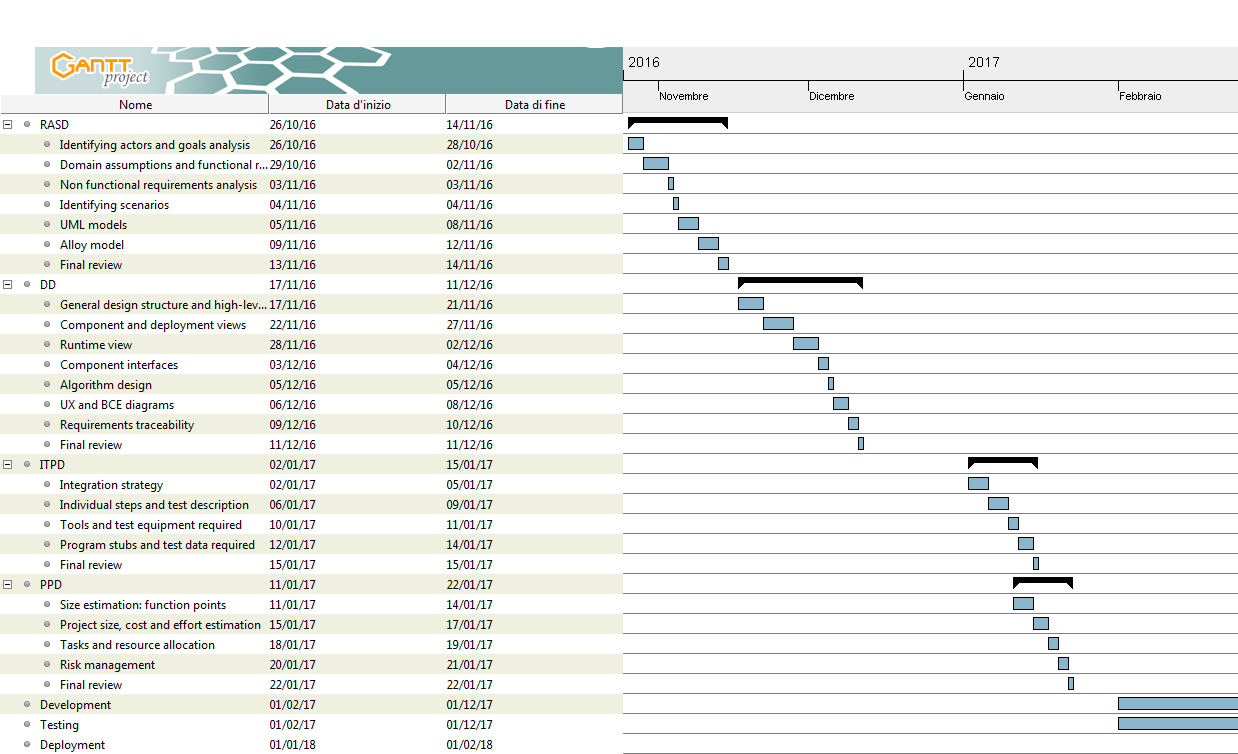
\includegraphics[width=1\textwidth]{Tasks1}
	\caption[Tasks-1]{The picture above shows the first section of Gantt chart representing main tasks of the project.}
	\label{fig:Tasks-1}
\end{figure}

\begin{figure}[H]
	\centering
	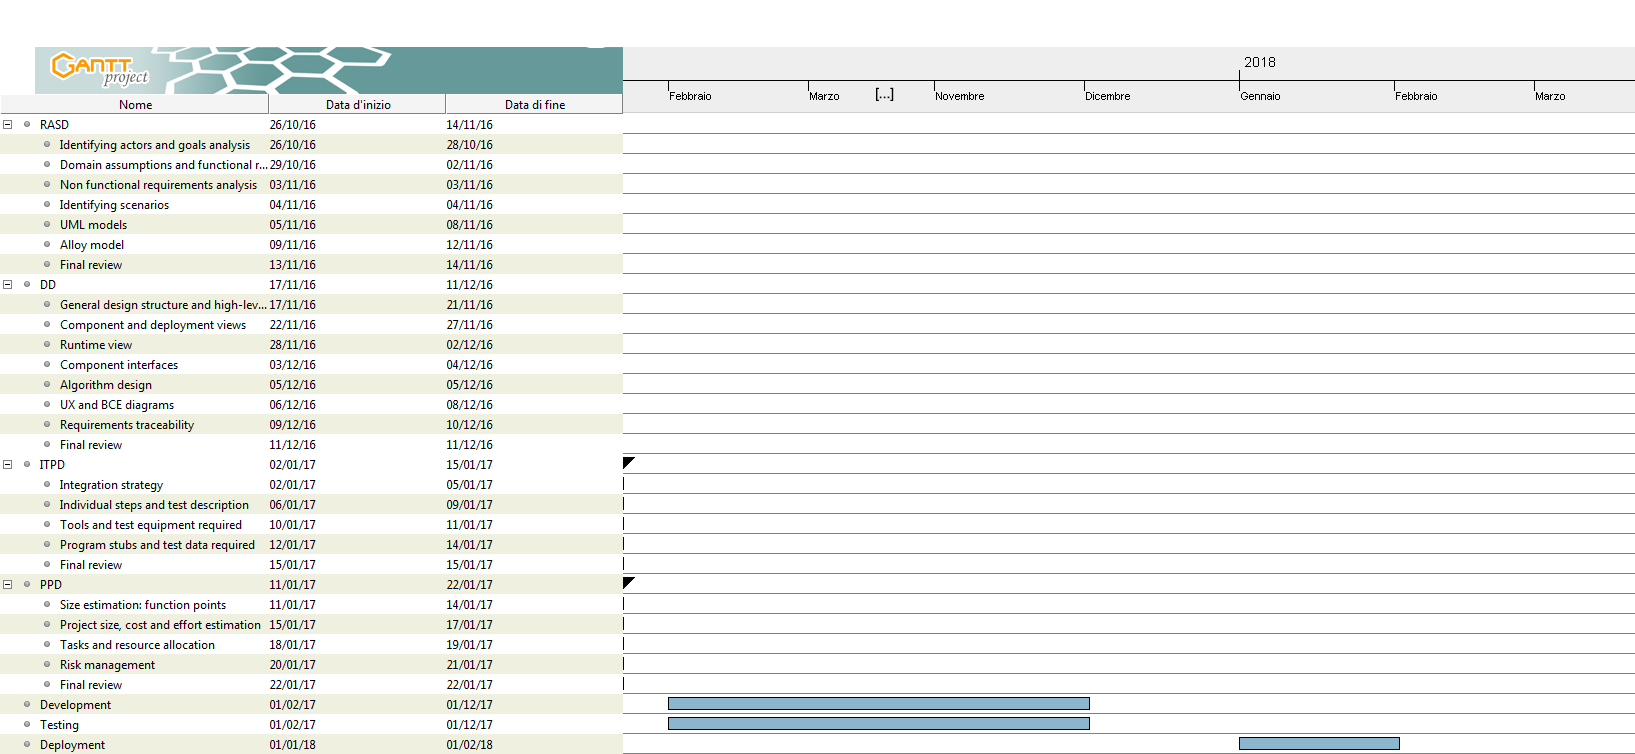
\includegraphics[width=1\textwidth]{Tasks2}
	\caption[Tasks-1]{The picture above shows the second section of Gantt chart representing main tasks of the project.}
	\label{fig:Tasks-2}
\end{figure}
%Resource Allocation
\chapter{Resource Allocation}
\blindtext

%Risk Management
% !TEX root = ../../../PPD/main.tex
\chapter{Risk Management}
In this Chapter, all the known risks related to planning, technical and business issues will be discussed. Along with the risks identified, a possible strategy to overcome them and to reduce the probability will be provided.

% Competition with other car-sharing companies
First of all, the most important risk that has been identified is the one related to the possible competition with other car sharing companies. Since at this time there are several companies that operates in the same cities where PowerEnJoy is expected to be deployed, it is important to evaluate all the possible scenarios related to this risk. The strategy to overcome this issue needs to be discussed with the marketing team. Well-planned marketing campaigns, interesting prices and services with respect to other companies and simple processes to learn how to use the service can be good strategies to adopt.

% Government sponsorship
Usually, projects that involves a service for the citizens are sponsored by local governments. It is fundamental to organize meeting with the local authorities in order to make them understand the importance and the benefits that PowerEnJoy would bring to the local communities. It is important to collect guarantees from the local governments about the expected economic investment in PowerEnJoy in order to deliver a complete and well designed product and to avoid wrong budget planning.

% Requirements volatility
Another risk is the one related to the requirements volatility. A thorough requirement elicitation phase is fundamental to collect all the projects specifications before taking any decision about the design or the implementation. PowerEnJoy is an application that can be expanded and integrated with multiple features. For this reason, it is important to come to an agreement with all the stakeholders before any development activities start.

% Modification or closing of the external services
Since PowerEnJoy relies on multiple external service, the malfunction, the modification or the closure of one of those would be a serious issue to deal with. The three main external services integrated in PowerEnJoy are the notification, payments and recovery service. Every services mentioned is fundamental for the correct functioning of the application. For this reason, a thorough investigation must be done in order to select the most reliable and known companies in each of those sectors.

% Deliver a user-friendly application
Although the overall process to take advantage of the PowerEnJoy services is intrinsically quite simple, the QA team must assure that the users will be able to easily learn how to use PowerEnJoy. If the users will face difficulties while approaching the app the first time, the effect could be catastrophic. The strategies that can be exploited to overcome this kind of risk are tests focused on the users, such as A/B and beta testing of the mobile and web application along with the interfaces of the onboard computers.

% Infrastructure reliability
PowerEnJoy must guarantee a 24/7 service. The possible downtimes that could happen if the infrastructure supporting PowerEnJoy would not be available represent a critical risk for the whole system. Important economic losses are expected if long downtimes happen. The strategy that can be applied is to make a thorough analysis of all the possible cloud providers in order to select the most suitable one for the system to be developed and deployed.

% Personnel Turnover and code understanding
Finally, the personnel turnover is a chance that must be considered. Serious delays of the system delivery must be expected if new developers join the project in the middle of the development process. As an example, a certain amount of time must be estimate to let the new employees learn the technologies that are used and how the already developed component works. To overcome this risk the personnel selection phase must be conduct with the right attention and the code base must be fully and high detailed documented.


\listoffigures
\begingroup
\let\clearpage\relax
\listoftables
\endgroup

\bibliographystyle{unsrt}
\bibliography{ref}

\end{document}
